\section{Signale und Systeme}
	\begin{tabular}{|l|l|}
    	\hline
    	\textbf{Linearität} & \textbf{Zeitinvarianz}\\
    	\hline
    	$S(x1+x2)=S(x1)+S(x2)$ & $S(x(t-t_0)=S(x)\cdot x(t-t_0)$ \\
    	$S(c\cdot x)=c\cdot S(x)$ & \\
		\hline    
    \end{tabular}
	
	\subsection{Lineare zeitinvariante Systeme (LTI-Systeme)}
		LTI-Systeme sind durch ihre Impulsantwort $h$ vollständig bestimmt\\ \\
		\textbf{Berechnung der Systemantwort von diskreten LTI-Systemen}\\
		$\; y=x*h \qquad$ ($y=$ Systemantwort; $x=$ Eingangssignal; $h=$
		Impulsantwort)\\
		
		\textbf{Berechnung der Systemantwort von kontinuierlichen LTI-Systemen}\\
		\begin{tabular}{ll}
			\parbox{8cm}{
			$$s_2(t) = h(t) * s_1(t) \laplace S_2(s) = H(s) S_1(s)$$
			$$h(t) \laplace H(s)$$}
			& \parbox{4cm}{
			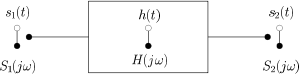
\includegraphics[width=5cm]{./bilder/utf-theorie.png}}\\
		\end{tabular}	
		
	\subsection{Faltung}
	\begin{tabular}{|l|} \hline
	$y(t) = f(t)\ast g(t) = g(t) \ast f(t) = (f \ast g)(t) :=
	\int\limits_{-\infty}^\infty f(u) \cdot g(t-u)\,du =
	\int\limits_{-\infty}^\infty f(t-u) \cdot h(u)\,du $ \\ \hline
	\end{tabular} \\
	
	Hat $g\left(t\right)$ keine negative Argumente dann gilt :
	$\left(g \ast f \right)\left(t\right)=\int\limits_{-\infty}^t f(u) \cdot
	g(t-u)\,du$\\
	Hat $f\left(t\right)$ keine negative Argumente (Einschaltvorgang) dann gilt :
	$\left(g \ast f \right)\left(t\right)=\int\limits_{0}^t f(u) \cdot
	g(t-u)\,du$\\
	Bei einer Faltung mit einer $\delta\left(t\right)$Funktion
	gilt:$f\left(t\right) \ast \delta\left(t\right) = f\left(t\right)$\\
	
	\begin{multicols}{2}
		\textbf{grafische Interpretation:}
		\begin{enumerate}
  			\item einfacheres Signal an der Y-Achse spiegeln
  			\item Verschiebung um t nach rechts
  			\item Multiplikation und Integration der beiden Signale
		\end{enumerate}
		\columnbreak
		\textbf{Bestimmung der Grenzen:}
		\begin{enumerate}
		  \item Koordinatensystem: X-Achse: t, Y-Achse: u
		  \item Erster Faktor $\rightarrow$ Streifen parallel zur X-Achse
		  \item Zweiter Faktor $\rightarrow$ Streiffen parallel zur $45^{\circ}$-Geraden
		  \item Grenzen für ein bestimmtes t ablesen
		\end{enumerate}
	\end{multicols}	

